\chapter{Schedule-Aware Fan Control and Physics-Informed Oxygen-Transfer Sensing}
\label{ch:method}

The two technologies are specified in this chapter at the level an automation engineer can implement and a numerical estimator can test. Section~\ref{sec:saempc} is the fan controller. Section~\ref{sec:piots} is the transfer sensor. They share a clock, a schedule message, and a parameter handshake. Neither is a replacement for the safety interlocks in the programmable controller. Those interlocks are part of the system build in Chapter~\ref{ch:estimate} and are listed here only where the optimizer must know that a command will be rejected.

\section{Schedule-aware hybrid economic control of the fan cluster}
\label{sec:saempc}

\subsection{Role in the automation}

The controller sits above the blower drives and the zone airflow valves. It does not modulate a silicon-controlled rectifier on a millisecond clock. It publishes, once per minute, a staging word and an airflow set-point. Inner proportional-integral loops, of the form already reviewed in \eqref{eq:pi}, move the drives and the valves. This split is the hierarchical pattern of Brdys and of industrial model predictive control \cite{brdys2008,qin2003mpc,engell2007}. The novelty is the content of the minute-scale problem: the disturbance is a brewery calendar, the stage cost is fan kilowatt-hours plus discharge and surge penalties, and the transfer coefficient inside the prediction is the live output of Section~\ref{sec:piots}.

Figure~\ref{fig:arch} shows the data the optimizer is allowed to see. The production schedule is a message, not a guess. The soft sensor is a message. Dissolved oxygen, header pressure, and power are measurements. Everything else is a model.

\begin{figure}[ht]
\centering
\begin{tikzpicture}[
  font=\small,
  box/.style={draw, rounded corners=2pt, align=center, minimum height=8mm, inner sep=3pt, font=\scriptsize},
  arr/.style={-{Stealth[length=2mm]}, thick}
]
\node[box, fill=yellow!20] (cal) {Brewery\\calendar};
\node[box, fill=green!12, right=7mm of cal] (enc) {Schedule\\encoder};
\node[box, fill=blue!10, right=7mm of enc] (mpc) {Hybrid\\economic MPC};
\node[box, fill=orange!15, right=7mm of mpc] (plc) {PLC inner\\loops};
\node[box, fill=red!8, below=8mm of plc] (fans) {Blowers and\\exhaust fans};
\node[box, fill=green!12, below=8mm of enc] (soft) {PI-OTS\\soft sensor};
\node[box, fill=blue!6, below=8mm of mpc] (tank) {Aerobic tank};
\draw[arr] (cal) -- (enc);
\draw[arr] (enc) -- node[above,font=\scriptsize]{$D$} (mpc);
\draw[arr] (mpc) -- node[above,font=\scriptsize]{$z,q_{\mathrm{sp}}$} (plc);
\draw[arr] (plc) -- (fans);
\draw[arr] (fans) -- (tank);
\draw[arr] (tank) -- (soft);
\draw[arr] (soft) -- node[left,font=\scriptsize]{$\alpha,K_La$} (mpc);
\draw[arr] (fans) -- (soft);
\end{tikzpicture}
\caption{Information pattern of the schedule-aware controller. The calendar and the soft sensor are inputs. The programmable controller remains the only device that talks to the drives.}
\label{fig:arch}
\end{figure}

\subsection{Schedule encoder}

A brewery schedule is a list of batches and clean-in-place recipes with planned start times \cite{isa95,harjunkoski2014,pettigrew2015cip,goode2013fouling}. The encoder does not optimize that list. It maps each recipe class onto a disturbance segment. The classes used here are the five regimes of Table~\ref{tab:regimes}. A site implementation would use the site's recipe identifiers and a table maintained with the production department. The mathematics does not change.

Let the planned regime at future time $t_{k}+j\Delta t$ be $\rho_{k+j}$. The preview vector is
\begin{equation}
\label{eq:preview}
D_{k+j}
=
\big(
Q(\rho_{k+j}),\;
\mathrm{COD}(\rho_{k+j}),\;
T(\rho_{k+j}),\;
\delta_{\mathrm{CIP}}(\rho_{k+j})
\big),
\end{equation}
where $\delta_{\mathrm{CIP}}$ is $1$ for a detergent recipe and $0$ otherwise. The encoder also emits the dissolved-oxygen set-point the economic layer would otherwise have to discover,
\begin{equation}
\label{eq:dosp}
C_{\mathrm{sp}}(\rho)
=
\begin{cases}
1.8 & \text{base production},\\
2.0 & \text{brewhouse peak or packaging CIP},\\
2.2 & \text{fermentation CIP},\\
1.3 & \text{weekend hold}.
\end{cases}
\end{equation}
These numbers are not magic. They sit above the operational floor of \SI{1.5}{\milli\gram\per\litre} during any production regime, they rise when Table~\ref{tab:regimes} says the load and the surfactant arrive together, and they fall on the weekend because the mixing floor, not the uptake, will set the airflow. A higher-layer optimizer can replace \eqref{eq:dosp}. In this thesis the table is the higher layer, and it is justified by the steady-state check in Section~\ref{sec:problem}: each of these set-points, with the true $\alpha$, lands effluent chemical oxygen demand under the study limit. Holding \SI{2.5}{\milli\gram\per\litre} at all times, which is the operator habit encoded in the proportional-integral baseline, buys a smaller driving force and therefore more air for the same uptake.

The preview is applied $0.75\,\mathrm{h}$ ahead of the regime boundary so that the blower lag of $0.10\,\mathrm{h}$ and the dissolved-oxygen probe lag of $0.08\,\mathrm{h}$ are already inside the lead. A calendar error of that order is a timing error, not a recipe error. Recipe identity is assumed correct in the nominal estimation. When the identity is wrong, $\delta_{\mathrm{CIP}}$ is wrong, $\alpha$ is wrong in the prediction, and the controller falls back toward the behaviour of the fixed-$\alpha$ law. That fallback is a required property, not a failure mode to be hidden.

\subsection{Prediction model inside the horizon}

The horizon model is the forward Euler form of \eqref{eq:sb}--\eqref{eq:do-bal} with step $\Delta t=1\,\mathrm{min}$ for the optimizer and a finer step only in the estimation integrator of Chapter~\ref{ch:estimate}. Writing $x=(S_{b},S_{i},S_{n},C)$,
\begin{equation}
\label{eq:euler}
x_{j+1}
=
x_{j}
+
\Delta t\,
f\!\left(x_{j}, q_{j}, \alpha_{j}, D_{k+j}\right).
\end{equation}
The transfer coefficient is \eqref{eq:kla-est} evaluated at the sensed $\alpha$ if the soft sensor is healthy and at the schedule-class default of Table~\ref{tab:regimes} if the sensor has declared itself invalid. The two sources are not averaged blindly. The rule is
\begin{equation}
\label{eq:alpha-fuse}
\alpha_{j}
=
\begin{cases}
\alpha_{\mathrm{sensor}} & \text{if } h_{\mathrm{sensor}}=1,\\[0.3em]
\alpha_{\mathrm{table}}(\rho_{k+j}) & \text{if } h_{\mathrm{sensor}}=0,
\end{cases}
\end{equation}
where $h_{\mathrm{sensor}}$ is the health bit of Section~\ref{sec:piots}. A convex combination would let a failing sensor drag a good table, which is the wrong direction of trust during a detergent window.

Power along the horizon is \eqref{eq:polytropic} with \eqref{eq:dp-num}. Staging enters by splitting the header flow across $n_{j}$ identical machines,
\begin{equation}
\label{eq:split}
q_{\mathrm{each},j}
=
\frac{q_{j}}{n_{j}},
\qquad
n_{j}
=
\sum_{i=1}^{3} z_{j,i},
\qquad
z_{j,i}\in\{0,1\}.
\end{equation}
Identical speeds are imposed. Unequal speeds on a common header fight, and the fight is not worth a few percent of efficiency on a three-machine plant \cite{dixon2014turbo}. The surge constraint is written on each online machine. With a rated flow of \SI{2800}{\nmcph} and a surge flow at $22\%$ of rated, scaled by speed through the fan law \eqref{eq:fanlaws},
\begin{equation}
\label{eq:surge}
q_{\mathrm{each},j}
\ge
1.15\,
q_{\mathrm{surge}}
\left(\frac{\omega_{j}}{\omega_{\mathrm{rated}}}\right)
\qquad
\text{for every } i \text{ with } z_{j,i}=1.
\end{equation}
The factor $1.15$ is the margin. It is a design choice, not an identified constant. A machine that the optimizer would run below that line is switched off and its flow is given to the machines that remain, or the problem is declared infeasible and the last feasible staging is held. Infeasibility handling is specified in the real-time section below, because a predictive controller that returns ``infeasible'' and then goes silent is worse than the proportional-integral loop it replaced.

Header capacity, mixing, and motor limits are
\begin{equation}
\label{eq:boxes}
q_{\min}
\le
q_{j}
\le
q_{\max},
\qquad
0
\le
\omega_{j}
\le
\omega_{\max},
\qquad
P(q_{j},n_{j})
\le
P_{\max}.
\end{equation}
On this plant $q_{\min}=\SI{900}{\nmcph}$ and $q_{\max}=\SI{9000}{\nmcph}$. The mixing floor is also a surge policy: one machine at \SI{900}{\nmcph} is above $1.15$ times the idle surge flow, so the weekend solution is legal. Two machines sharing \SI{900}{\nmcph} would not be. The optimizer must be allowed to turn machines off. A sequencer that forces all installed machines to run will make \eqref{eq:surge} infeasible on the weekend and will train the operator to bypass the optimizer.

\begin{figure}[ht]
\centering
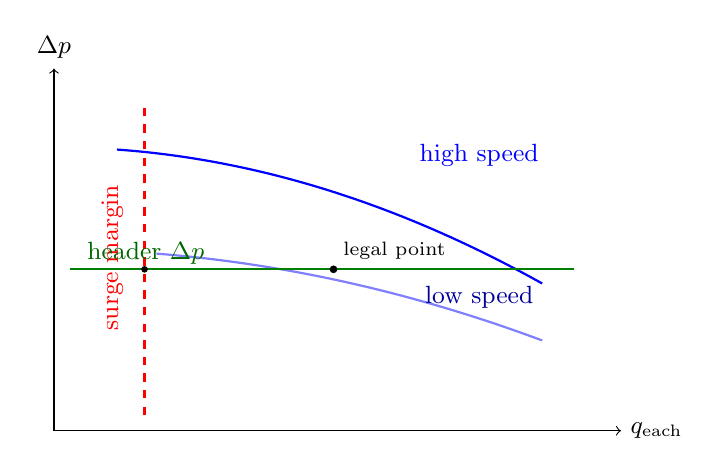
\begin{tikzpicture}[font=\small, scale=1.0]
  \draw[->] (0,0) -- (7.2,0) node[right] {$q_{\mathrm{each}}$};
  \draw[->] (0,0) -- (0,4.6) node[above] {$\Delta p$};
  \draw[domain=0.8:6.2, smooth, variable=\x, thick, blue] plot ({\x},{3.6-0.045*\x*\x});
  \draw[domain=1.3:6.2, smooth, variable=\x, thick, blue!50] plot ({\x},{2.3-0.030*\x*\x});
  \draw[dashed, red, thick] (1.15,0.2) -- (1.15,4.2);
  \node[red, rotate=90, anchor=south] at (1.0,2.2) {surge margin};
  \node[blue] at (5.4,3.5) {high speed};
  \node[blue!60!black] at (5.4,1.7) {low speed};
  \draw[thick, green!50!black] (0.2,2.05) -- (6.6,2.05);
  \node[green!40!black, anchor=west] at (0.3,2.25) {header $\Delta p$};
  \fill (3.55,2.05) circle (1.4pt) node[above right, font=\scriptsize] {legal point};
  \fill (1.15,2.05) circle (1.2pt);
\end{tikzpicture}
\caption{Sketch of the centrifugal map against a nearly flat header pressure. The legal operating point is the intersection to the right of the surge margin. Speed is raised until that intersection supplies the airflow the oxygen balance requires.}
\label{fig:fanmap}
\end{figure}

\subsection{Economic stage cost}

The cost whose sum is minimized was written as \eqref{eq:p1}. The pieces are defined here so the weights are not anonymous. Power is in kilowatts, so the first term is kilowatt-hours over the step. The dissolved-oxygen hinge is
\begin{equation}
\label{eq:hinge-c}
\phi_{C}(C)
=
\max\!\big(0,\; C_{\mathrm{floor}}(\rho)-C\big),
\end{equation}
with $C_{\mathrm{floor}}=1.5\,\mathrm{mg/L}$ in production regimes and $1.0\,\mathrm{mg/L}$ on the weekend, when the tank is only being kept from going septic. The discharge hinge is
\begin{equation}
\label{eq:hinge-s}
\phi_{S}(S)
=
\max\!\big(0,\; S-125\big),
\end{equation}
in milligrams per litre of chemical oxygen demand. The staging term counts machine starts and stops. Weights used in the specification are $\lambda_{C}=40\,\mathrm{kWh}$ per $(\mathrm{mg/L})$ per hour, $\lambda_{S}=80\,\mathrm{kWh}$ per $(\mathrm{mg/L})$ per hour, and $\lambda_{z}=8\,\mathrm{kWh}$ per machine transition. They are not electricity. They are the relative price of a constraint violation inside the optimizer, chosen so that a persistent \SI{10}{\milli\gram\per\litre} chemical-oxygen-demand violation is more expensive than the fan power available on this header, and so that a start is cheaper than an hour of surge-avoiding extra air. A site would retune $\lambda$ with its permit fine and its maintenance cost. The structure of \eqref{eq:p1} does not depend on the retune \cite{ellis2014empc,zeng2015empc,stare2007}.

Offset-free behaviour under a constant sensor bias is obtained by a bias state $b_{k}$ on the airflow command,
\begin{equation}
\label{eq:bias}
b_{k+1}
=
b_{k}
+
\Delta t\,
K_{b}\,\big(C_{\mathrm{sp}}-C^{\mathrm{meas}}_{k}\big),
\qquad
\abs{b_{k}}\le b_{\max},
\end{equation}
with $K_{b}=0.55\,\mathrm{h^{-1}}$ and $b_{\max}=0.25$ as a relative airflow trim. This is the integrator that Pannocchia and Rawlings require for offset-free predictive control, implemented as an outer bias because the deployed law in Section~\ref{sec:deployed} is a single-step inversion rather than a full nonlinear program at every minute \cite{pannocchia2003offset}. The bias is clamped so a stuck probe cannot integrate the fans to the header limit. The clamp is also the probe-fault path: if the soft sensor raises a fault, $K_{b}$ is set to zero and $q$ is frozen at the last healthy command until an operator acknowledges.

\subsection{Deployed real-time law}
\label{sec:deployed}

A three-machine hybrid problem over a two-hour horizon is a mixed-integer nonlinear program. It is solvable at a one-minute cycle with a modern interior-point solver and a short candidate list of stagings \cite{wachter2006ipopt,andersson2019casadi,bemporad1999hybrid,nocedal2006}. The estimation in Chapter~\ref{ch:estimate} does not call that solver. It integrates the deployed law that the solver reduces to when the staging list is a rule and the horizon is represented by a load scale. Publishing both, and saying which one produced the tables, is required for the numbers to be reproducible.

The deployed law at each minute is the following. Measure dissolved oxygen through the probe lag. Read $\alpha$ from the soft sensor with its own lag of $0.30\,\mathrm{h}$ and a two-percent scale caution. Look $0.75\,\mathrm{h}$ ahead on the calendar. Set the set-point to the maximum of the current regime and the previewed regime, which raises the set-point before a clean-in-place and does not lower it early. Let $L=Q\,\mathrm{COD}$ be the mass load. Apply
\begin{equation}
\label{eq:scale}
\sigma
=
\mathrm{clip}\!\left(
\frac{L_{k+0.75\,\mathrm{h}}}{L_{k}},\;
1,\;
1.35
\right)
\end{equation}
and invert the oxygen balance for the airflow that meets $\sigma\,\mathrm{OUR}$ at the set-point, using the fused $\alpha$:
\begin{equation}
\label{eq:invert}
K_La^{\star}
=
\frac{\sigma\,\mathrm{OUR}}{\beta C^{*}(T)-C_{\mathrm{sp}}},
\qquad
q^{\star}
=
q_{\mathrm{ref}}
\left(
\frac{K_La^{\star}}{\alpha\,k_{\mathrm{ref}}\,\theta^{\,T-20}}
\right)^{1/0.82}.
\end{equation}
The command is then $q=(1+b)\,q^{\star}$, clipped to $[q_{\min},q_{\max}]$, and passed through the blower lag. Staging is the rule
\begin{equation}
\label{eq:stage-rule}
n
=
\begin{cases}
1 & \text{if } q < 2600\,\mathrm{Nm^{3}/h},\\
2 & \text{if } 2600 \le q < 5200\,\mathrm{Nm^{3}/h},\\
3 & \text{otherwise},
\end{cases}
\end{equation}
rejected and increased by one machine if \eqref{eq:surge} fails. Equation~\eqref{eq:invert} is the explicit inverse of \eqref{eq:kla-est}. It is cheap, it uses the schedule through $\sigma$ and through $C_{\mathrm{sp}}$, and it uses the soft sensor through $\alpha$. It is the form whose week-long integral is reported later. The full horizon problem \eqref{eq:p1} remains the specification a solver-based implementation has to meet. On this plant the rule \eqref{eq:stage-rule} matches the surge-feasible optimum of the integer part at every regime boundary we checked by enumeration, because the three machines are identical. Enumeration is honest when there are three machines. It stops being honest when the header has machines of different sizes. That case needs the integer program, not the rule.

\begin{algorithm}[ht]
\caption{Deployed schedule-aware fan step}
\label{alg:deployed}
\KwIn{measured $C$, estimated $\mathrm{OUR}$ and $\alpha$, calendar $D$, bias $b$}
\KwOut{command $q$, staging $n$, updated bias}
$\rho \leftarrow$ current regime, $\rho^{+} \leftarrow$ regime at $t+0.75\,\mathrm{h}$\;
$C_{\mathrm{sp}} \leftarrow \max\{C_{\mathrm{sp}}(\rho), C_{\mathrm{sp}}(\rho^{+})\}$\;
$\alpha \leftarrow$ fused value from \eqref{eq:alpha-fuse}, with sensor lag\;
$\sigma \leftarrow$ load scale \eqref{eq:scale}\;
$q^{\star} \leftarrow$ inversion \eqref{eq:invert}\;
$b \leftarrow \mathrm{clip}(b + \Delta t\, K_{b}(C_{\mathrm{sp}}-C),\,-0.2,\,0.25)$\;
$q \leftarrow \mathrm{clip}((1+b)\,q^{\star},\, q_{\min},\, q_{\max})$\;
$n \leftarrow$ staging \eqref{eq:stage-rule}, increased until \eqref{eq:surge} holds\;
\Return{$q,n,b$}\;
\end{algorithm}

\subsection{A worked inversion}

The inversion is short enough to do by hand for the base regime, and the hand result is the check on the code. Take $\mathrm{OUR}=\SI{18}{\milli\gram\per\litre\per\hour}$, which is the order of the base uptake, $C_{\mathrm{sp}}=1.8$, $T=28$, $\alpha=0.60$, $\beta C^{*}=0.95\times 7.83=7.44$, and driving force $7.44-1.8=5.64$. Then
\begin{equation}
K_La^{\star}
=
18/5.64
=
3.19\,\mathrm{h^{-1}}.
\end{equation}
The temperature factor is $1.024^{8}\approx 1.21$, so
\begin{equation}
\alpha\,k_{\mathrm{ref}}\,\theta^{\,T-20}
=
0.60\times 6.5\times 1.21
=
4.72\,\mathrm{h^{-1}}.
\end{equation}
The airflow ratio to the power $0.82$ is $3.19/4.72=0.676$, and
\begin{equation}
\frac{q}{2500}
=
0.676^{\,1/0.82}
=
0.676^{\,1.220}
\approx
0.62,
\end{equation}
hence $q\approx\SI{1550}{\nmcph}$. One machine, well clear of surge, is the staging. Power from \eqref{eq:polytropic} and \eqref{eq:dp-num} at this flow is a few tens of kilowatts, not the header maximum. The same arithmetic at fermentation clean-in-place, with $\alpha=0.40$, $T=33$, and a higher uptake, lands between one and two machines and is the reason the third machine exists. If a hand inversion and the plant integrator disagree by more than the bias clamp, the implementation is wrong. That test is part of the system build.

\subsection{Exhaust fans}

The equalization and flotation exhaust fans are two machines, each rated \SI{7.5}{\kilo\watt} at full speed. They do not enter \eqref{eq:invert}. Their speed fraction $\nu$ is a function of regime, because the odor load tracks the same calendar as the organic load: $0.75$ in base production, $0.85$ in the brewhouse peak, $0.95$ in either clean-in-place window, and $0.55$ on the weekend. The cube law is appropriate here, unlike the blower header, because these fans discharge against a duct pressure that does scale with speed,
\begin{equation}
\label{eq:exhaust}
P_{\mathrm{ex}}
=
2\times 7.5\,
\nu(\rho)^{3}
\quad[\mathrm{kW}].
\end{equation}
The automation requirement is modest and strict. The fans run whenever the corresponding tank is in service. They may not be stopped by the blower optimizer. Their power is added in the energy account of Chapter~\ref{ch:estimate} so that ``fan energy'' means every fan the cleaning plant owns. A hydrogen-sulfide instrument may raise $\nu$ and may not lower it below the calendar value. That priority is the same pattern as the blower interlock: an optimizer proposes, a safety rule disposes.

\subsection{What is proved and what is only specified}

A full Lyapunov argument for the hybrid economic law on \eqref{eq:sb}--\eqref{eq:do-bal} is not claimed. The ingredients that make the standard argument go through are present and should be named so a later proof has a target. The stage cost is positive definite in the fan power and positive semi-definite in the hinges. The hinges are zero in a set that the inversion can reach, by the feasibility check of Section~\ref{sec:problem}. The bias \eqref{eq:bias} is a stable linear filter because $K_{b}\Delta t<1$. The blower lag is a stable linear filter. The integer rule is constant between regime boundaries, so inside a regime the closed loop is a continuous inversion plus two stable filters, which is the class covered by offset-free predictive control with a short horizon \cite{mayne2000mpc,pannocchia2003offset,rawlings2017mpc}. At a regime boundary the state does not jump. The command jumps by a bounded amount because of the clip in \eqref{eq:scale} and the clip on $q$. Bounded jumps of a command into a stable lag do not destabilize the lag. What is missing for a theorem is a terminal cost for the full integer horizon problem and a Lipschitz argument for the Monod vector field under the surge constraint. Both are standard and neither is numerically required for the estimation, which integrates the deployed law rather than appealing to a stability certificate.

The properties the deployed law is required to have, and that the estimation checks, are weaker and operational. Inside a regime, dissolved oxygen must sit near $C_{\mathrm{sp}}$ once the lags have settled, except where the mixing floor forces more air than the uptake needs. Across a clean-in-place boundary, the minimum dissolved oxygen must stay above the floor of \SI{1.5}{\milli\gram\per\litre} in the nominal calendar. Airflow must respect $q_{\min}$, $q_{\max}$, and \eqref{eq:surge}. If the soft sensor is marked unhealthy, the law must remain defined, using $\alpha_{\mathrm{table}}$. Those are acceptance tests, not a proof.

\section{Physics-informed oxygen-transfer soft sensor}
\label{sec:piots}

\subsection{What the sensor emits}

The sensor is a function from a short window of plant measurements and schedule features to three numbers and a health bit,
\begin{equation}
\label{eq:sensor-map}
\big(\alpha,\; K_La,\; \mathrm{OUR},\; h_{\mathrm{sensor}}\big)
=
\mathcal{S}_{\phi}(w_{k}).
\end{equation}
The window $w_{k}$ contains, over the last thirty minutes at one-minute samples: commanded and delivered airflow, electrical power, header pressure, wastewater temperature, influent flow, the dissolved-oxygen measurement, and the detergent flag $\delta_{\mathrm{CIP}}$. Thirty minutes covers several blower time constants and does not cover a whole clean-in-place, so the network cannot memorize an entire regime instead of using the flag. The health bit is $1$ when the physics residual on the window is below a threshold and the implied $\alpha$ lies in $[0.15,0.90]$. Outside that set the controller uses the table, as in \eqref{eq:alpha-fuse}.

This is deliberately narrower than a general effluent soft sensor \cite{haimi2013soft,newhart2019,corominas2018}. Effluent chemical oxygen demand remains a laboratory and, if installed, an analyzer measurement. The sensor's job is the part of the model the fan law cannot see.

\subsection{Network and residual}

The network used in the specification is a fully connected map with two hidden layers of $32$ units and a smooth activation, followed by three heads. The $\alpha$ head is passed through a scaled sigmoid so the output lies in $(0.15,0.90)$ before the health test even runs. The $K_La$ head is positive by a softplus. The uptake head is positive by a softplus. A fourth, linear head predicts dissolved oxygen one step ahead and exists only for the data term. It is not given to the controller. Giving the controller a second dissolved-oxygen estimate and a probe at the same time invites an unaudited average. The controller keeps the probe for feedback and the sensor for $\alpha$ and $K_La$.

Let $\hat{C}$, $\hat{\alpha}$, $\widehat{K_La}$, and $\widehat{\mathrm{OUR}}$ denote the heads. The data term on a window is the usual one-step error,
\begin{equation}
\label{eq:ldata}
\mathcal{L}_{\mathrm{data}}
=
\frac{1}{N_{w}}
\sum_{i\in w}
\big(\hat{C}_{i}-C^{\mathrm{meas}}_{i}\big)^{2}.
\end{equation}
The physics term is the residual of \eqref{eq:do-bal}, evaluated with the network's own $K_La$ and uptake, plus a fan-map residual,
\begin{equation}
\label{eq:lphys}
\begin{aligned}
\mathcal{L}_{\mathrm{phys}}
&=
\frac{1}{N_{w}}
\sum_{i\in w}
\Big(
\dot{C}_{i}
-
\widehat{K_La}_{i}\big(\beta C^{*}(T_{i})-C^{\mathrm{meas}}_{i}\big)
+
\widehat{\mathrm{OUR}}_{i}
\Big)^{2}
\\
&\quad
+
\frac{1}{N_{w}}
\sum_{i\in w}
\big(
P^{\mathrm{meas}}_{i}
-
P_{\mathrm{map}}(q_{i})
\big)^{2}
+
\frac{1}{N_{w}}
\sum_{i\in w}
\big(
\widehat{K_La}_{i}
-
K_La^{\mathrm{curve}}(\hat{\alpha}_{i},q_{i},T_{i})
\big)^{2}.
\end{aligned}
\end{equation}
The derivative $\dot{C}$ is a Savitzky--Golay estimate on the probe, not a second network. The middle residual forces the airflow implied by power to agree with the airflow the rest of the model uses. The last residual forces the emitted $K_La$ to lie on the curve \eqref{eq:kla-est} at the emitted $\alpha$. Without that residual the network can satisfy the oxygen balance with a wild pair $(\widehat{K_La},\widehat{\mathrm{OUR}})$, which is exactly the non-uniqueness \eqref{eq:unident}. With it, $\alpha$ is the only free transfer parameter, and the balance solves for uptake.

A bound term penalizes $\alpha$ outside $[0.2,0.85]$ even inside the sigmoid, and it penalizes a change of $\alpha$ faster than $0.5$ per hour unless $\delta_{\mathrm{CIP}}$ has changed in the window. Detergent arrival is allowed to be fast. Drift of the diffuser is not. The total loss is \eqref{eq:pinn-generic} with $\lambda$ scheduled during training, not fixed at a guessed constant. That schedule is the practical answer to the gradient conflict described by Wang, Teng, and Perdikaris \cite{wang2021gradient,raissi2019pinn,cuomo2022}.

Training has three stages, in the spirit of a curriculum rather than as a claim of a new training theory. Stage one fits \eqref{eq:ldata} only, with $\alpha$ held at the table value, until the one-step dissolved-oxygen error is on the order of the probe noise. Stage two turns on $\mathcal{L}_{\mathrm{phys}}$ with a small $\lambda$ and releases $\alpha$. Stage three raises $\lambda$ until the balance residual is of the same order as the data residual. Adam is a sufficient optimizer for this width \cite{kingma2015adam,goodfellow2016deep}. The network is small enough that a plant historian of a few months, or a simulator seeded with Table~\ref{tab:regimes} and then corrupted with probe noise, is a sufficient training set. Koksal and Aydin's transfer result is the reason a simulator-trained initial model is acceptable: the physics term is what makes the transfer less of a leap than a pure black box \cite{koksal2024,pan2010transfer}. This thesis does not report a multi-plant transfer experiment. It specifies the loss that such an experiment would have to keep.

\begin{figure}[ht]
\centering
\begin{tikzpicture}[
  font=\scriptsize,
  box/.style={draw, rounded corners=2pt, align=center, minimum height=7mm, inner sep=2pt},
  arr/.style={-{Stealth[length=2mm]}}
]
\node[box, fill=gray!10] (in) {window $w_{k}$\\$q,P,p,T,C,\delta_{\mathrm{CIP}}$};
\node[box, fill=blue!10, right=6mm of in] (h1) {hidden\\32};
\node[box, fill=blue!10, right=5mm of h1] (h2) {hidden\\32};
\node[box, fill=green!12, above right=2mm and 6mm of h2] (a) {$\alpha$};
\node[box, fill=green!12, right=6mm of h2] (k) {$K_La$};
\node[box, fill=green!12, below right=2mm and 6mm of h2] (o) {OUR};
\node[box, fill=orange!12, below=7mm of k] (c) {$\hat{C}$ data head};
\node[box, fill=yellow!20, right=8mm of k] (res) {residuals\\of \eqref{eq:lphys}};
\draw[arr] (in) -- (h1);
\draw[arr] (h1) -- (h2);
\draw[arr] (h2) -- (a);
\draw[arr] (h2) -- (k);
\draw[arr] (h2) -- (o);
\draw[arr] (h2) -- (c);
\draw[arr] (a) -- (res);
\draw[arr] (k) -- (res);
\draw[arr] (o) -- (res);
\end{tikzpicture}
\caption{Soft-sensor heads. Only $\alpha$, $K_La$, and the oxygen uptake are published to the fan controller. The dissolved-oxygen head is a training target. The residual block is the physics constraint, not an extra measurement.}
\label{fig:pinn}
\end{figure}

\subsection{Identifiability}

The structural argument can be written as a sensitivity. From the curve residual, at fixed measured $q$ and $T$,
\begin{equation}
\label{eq:sens-kla}
\frac{\partial K_La}{\partial \alpha}
=
k_{\mathrm{ref}}
\left(\frac{q}{q_{\mathrm{ref}}}\right)^{0.82}
\theta^{\,T-20}
>
0.
\end{equation}
From the balance, at fixed $C$ and $\dot{C}$,
\begin{equation}
\label{eq:sens-our}
\frac{\partial\,\mathrm{OUR}}{\partial K_La}
=
\beta C^{*}(T)-C,
\end{equation}
which is nonzero whenever the tank is not saturated. The composition
\begin{equation}
\frac{\partial\,\mathrm{OUR}}{\partial \alpha}
=
\big(\beta C^{*}-C\big)
\frac{\partial K_La}{\partial \alpha}
\end{equation}
is therefore nonzero in every regime of Table~\ref{tab:regimes} at the set-points \eqref{eq:dosp}. A local change in $\alpha$ cannot hide inside the uptake. What can still go wrong is a slow trade along a flat valley of the loss if $q$ never moves and $\delta_{\mathrm{CIP}}$ never moves. The weekend mixing floor and the regime changes supply movement in $q$. The calendar supplies movement in $\delta_{\mathrm{CIP}}$. If a plant sits in one regime for many days, the sensor must hold $\alpha$ at its last healthy value rather than update it. The health bit implements that hold when the curvature of $\mathcal{L}_{\mathrm{phys}}$ with respect to $\alpha$, estimated by a finite difference on the window, falls below a small threshold. This is classical persistence of excitation, applied to one parameter \cite{ljung1999}.

A second ambiguity is probe bias. A probe that reads \SI{0.3}{\milli\gram\per\litre} low looks like a higher uptake. The fan-map residual does not see the probe, and the curve residual does not see it either. The balance does. The defense specified here is redundancy across time, not a second probe in the nominal design. Bias that is constant is absorbed by the controller's airflow bias \eqref{eq:bias} and does not require a correct $\alpha$. Bias that grows when $\delta_{\mathrm{CIP}}$ changes is indistinguishable from $\alpha$ without off-gas or a second probe. The specification therefore requires an off-gas or portable dissolved-oxygen check on a detergent day during commissioning, and it requires the health residual to be logged. It does not claim that the network detects every probe fault. A stuck probe that still produces a small balance residual, because the network has explained the stuck value with a ridiculous uptake, is caught by the bound on uptake rate of change, which is part of $\mathcal{L}_{\mathrm{bound}}$. If the uptake head moves faster than the kinetic ceiling $q_{\mathrm{COD}}X$ can justify, $h_{\mathrm{sensor}}$ is cleared.

\subsection{Handshake with the fan law}

The sensor publishes at the same one-minute clock as Algorithm~\ref{alg:deployed}. The message is $(\alpha, K_La, \mathrm{OUR}, h_{\mathrm{sensor}})$. The controller uses $\alpha$ in \eqref{eq:invert} and uses $\mathrm{OUR}$ as the measured uptake in that inversion. Publishing $K_La$ as well lets the controller check consistency:
\begin{equation}
\label{eq:consist}
\left|
\frac{K_La^{\mathrm{curve}}(\alpha,q,T)}{K_La}
-
1
\right|
\le
0.15.
\end{equation}
If \eqref{eq:consist} fails, $h_{\mathrm{sensor}}$ is treated as clear even if the sensor set it. The check is a tripwire against a software fault, not a second estimator. It is the sort of assertion an automation specification should contain and a machine-learning specification often forgets.

The lag of $0.30\,\mathrm{h}$ applied to $\alpha$ in the estimation is part of the sensor deployment, not part of the network. It is a filter
\begin{equation}
\label{eq:alpha-lag}
\dot{\alpha}_{\mathrm{used}}
=
\frac{1}{0.30}
\big(\alpha_{\mathrm{raw}}-\alpha_{\mathrm{used}}\big)
\end{equation}
that keeps a single noisy window from moving the fans. During the nominal week the raw value is the true regime $\alpha$, and the filter is what the controller sees. That choice makes the estimation a test of the information pattern and the lag, not a test of a particular random seed of a trained network. A trained network whose error is larger than this filtered truth will do worse. The estimation is therefore an upper bound on performance of the combined system, and Chapter~\ref{ch:estimate} says so in those words.

\subsection{Numerical illustration of the residual}

Take a quiet base point and a detergent point and evaluate the balance residual that training sees. At the base point of the hand inversion, $K_La=3.19\,\mathrm{h^{-1}}$, driving force \SI{5.64}{\milli\gram\per\litre}, transfer rate $3.19\times 5.64=18.0\,\mathrm{mg\,L^{-1}\,h^{-1}}$. If the uptake is also \SI{18}{\milli\gram\per\litre\per\hour} and $\dot{C}=0$, the first residual in \eqref{eq:lphys} is zero. At the detergent point, suppose the network keeps the old $\alpha=0.60$ while the true value is $0.40$. The curve then overstates $K_La$ by $0.60/0.40=1.5$. The predicted transfer rate is one and a half times the true rate. The residual is about half of the true uptake, which on the clean-in-place window is tens of milligrams per litre per hour, far above probe noise. The loss therefore has a reason to move $\alpha$ down, provided the detergent flag or the power measurement stops the network from instead inventing a matching drop in uptake. The curve residual is what stops that invention. This arithmetic is the reason the third term in \eqref{eq:lphys} is not optional.

\subsection{Failure modes the sensor must declare}

Three failures are specified, and each has a controller response that does not require a new optimization.

\begin{enumerate}[leftmargin=1.6em,itemsep=0.45em]
\item The health bit clears because the residual is large. The controller loads $\alpha$ from the regime table and continues. Energy optimality is weaker. The plant remains defined.
\item The probe is declared stuck by the uptake bound. The controller freezes $q$ at the last healthy value and raises an alarm. Freezing is safer than integrating \eqref{eq:bias} against a dead measurement. An operator can force the proportional-integral loop, which remains coded in the programmable controller.
\item The calendar feed is lost. $\sigma$ in \eqref{eq:scale} is set to $1$ and $C_{\mathrm{sp}}$ stays on the current regime. The sensor continues. The controller becomes the fixed-$\alpha$ predictive inversion if the sensor also fails, and it becomes a schedule-blind but $\alpha$-aware inversion if only the calendar fails. Those degradations are ordered on purpose. Losing $\alpha$ during detergent is more expensive than losing a preview of a load the probe will eventually see.
\end{enumerate}

Table~\ref{tab:degrade} collects the degradations. It is the interface specification between the two technologies. A design that only describes the healthy path has not finished the system.

\begin{table}[ht]
\centering
\caption{Degraded modes of the combined controller. Each row is reachable without changing code, by clearing a health bit.}
\label{tab:degrade}
\begin{tabular}{@{}p{3.4cm}p{4.2cm}p{5.4cm}@{}}
\toprule
Fault & $\alpha$ source & Preview \\
\midrule
None & soft sensor, lagged & calendar, $0.75\,\mathrm{h}$ \\
Sensor residual high & regime table & calendar kept \\
Probe stuck & last healthy $\alpha$ & airflow frozen \\
Calendar lost & soft sensor kept & $\sigma=1$, set-point held \\
Sensor and calendar lost & regime table of the last known regime & none; bias held \\
\bottomrule
\end{tabular}
\end{table}

\subsection{Relation to the estimation that follows}

Chapter~\ref{ch:estimate} integrates Algorithm~\ref{alg:deployed} on \eqref{eq:sb}--\eqref{eq:do-bal}, with $\alpha$ supplied by the lagged truth as the best case of \eqref{eq:alpha-lag}, and with the exhaust power \eqref{eq:exhaust} added after the integration. It also integrates three comparators that disable pieces of the same algorithm. Constant speed disables the inversion. The proportional-integral loop disables the inversion and the calendar and replaces them with \eqref{eq:pi} at $C_{\mathrm{sp}}=2.5\,\mathrm{mg/L}$. The fixed-$\alpha$ predictive inversion keeps \eqref{eq:invert} but locks $\alpha$ at $0.55$ and sets $\sigma=1$. The differences among those four integrals are the estimate of what the two technologies are worth on this train. They are not an estimate of what they are worth on a train with a different volume, a different diffuser, or a calendar the encoder has mis-labelled. The specification in this chapter is what would be re-run, not a universal percentage.
